\documentclass[10pt]{nsibeamer}
\title{Chapitre 03 : Bases de données}
\subtitle{Partie 2}
\author{NSI2}
\begin{document}
	\maketitle
    \section{Niveau logique\\ Modèle relationnel}
\begin{frame}{Principe}
On adapte un MCD en tables à deux dimensions.\\
On décide du type des attributs.\\
Pour l'instant, on peut utiliser des types génériques, qui sont susceptibles de varier légèrement d'un SGBD à un autre :
\begin{itemize}
	\item	\mintinline{sql}{INTEGER} pour les entiers;
	\item	\mintinline{sql}{FLOAT} ou \mintinline{sql}{REAL} pour les nombres en virgule flottante;
    \item	\mintinline{sql}{VARCHAR(taille)} ou \mintinline{sql}{TEXT} pour les chaînes de caractères de taille fixe ou illimitée;
    \item 	\mintinline{sql}{BIT} pour les booléens;
    \item 	\mintinline{sql}{DATE} et \mintinline{sql}{TIME} pour les heures et les dates;
\end{itemize}
\end{frame}


\begin{frame}{Transformer une entité en relation}
	On va transformer chaque entité du MCD en \alert{relation} :
	\begin{center}
		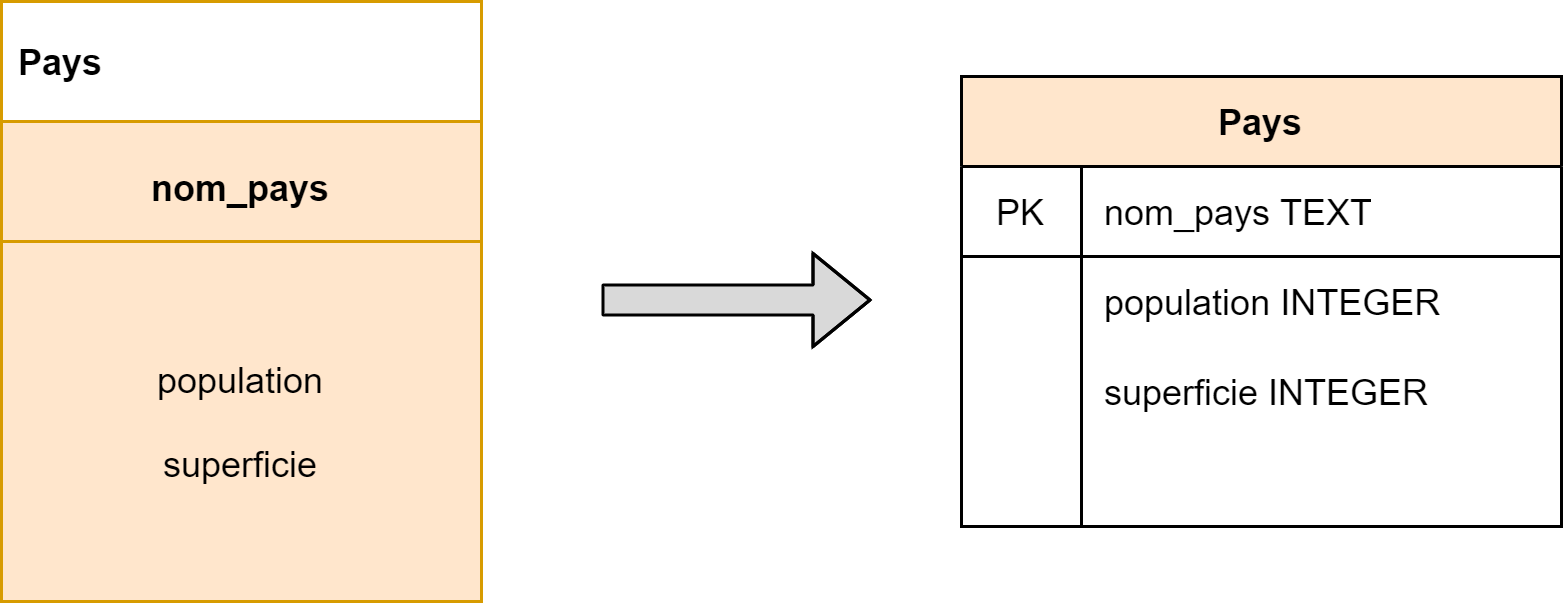
\includegraphics[width=7cm]{img/entite_vers_relation}
	\end{center}
	On indique les types de chaque attribut de la relation.

	Le ou les identifiants de l'entité sont appelés des \alert{clés primaires} pour la relation : « PK» est l'abréviation de \mintinline{sql}{PRIMARY KEY}.\\
	Le nom de la relation est noté en gras, la clé primaire soulignée.\\

	\textbf{Pays}(\uline{nom\_pays TEXT}, population INTEGER, superficie INTEGER)\\
\end{frame}



\begin{frame}{Transformer une association en relation : cas (0,1) ou (1,1)}
	\alert{Quand la relation possède une cardinalité valant (0,1) ou (1,1)}
	\begin{center}
		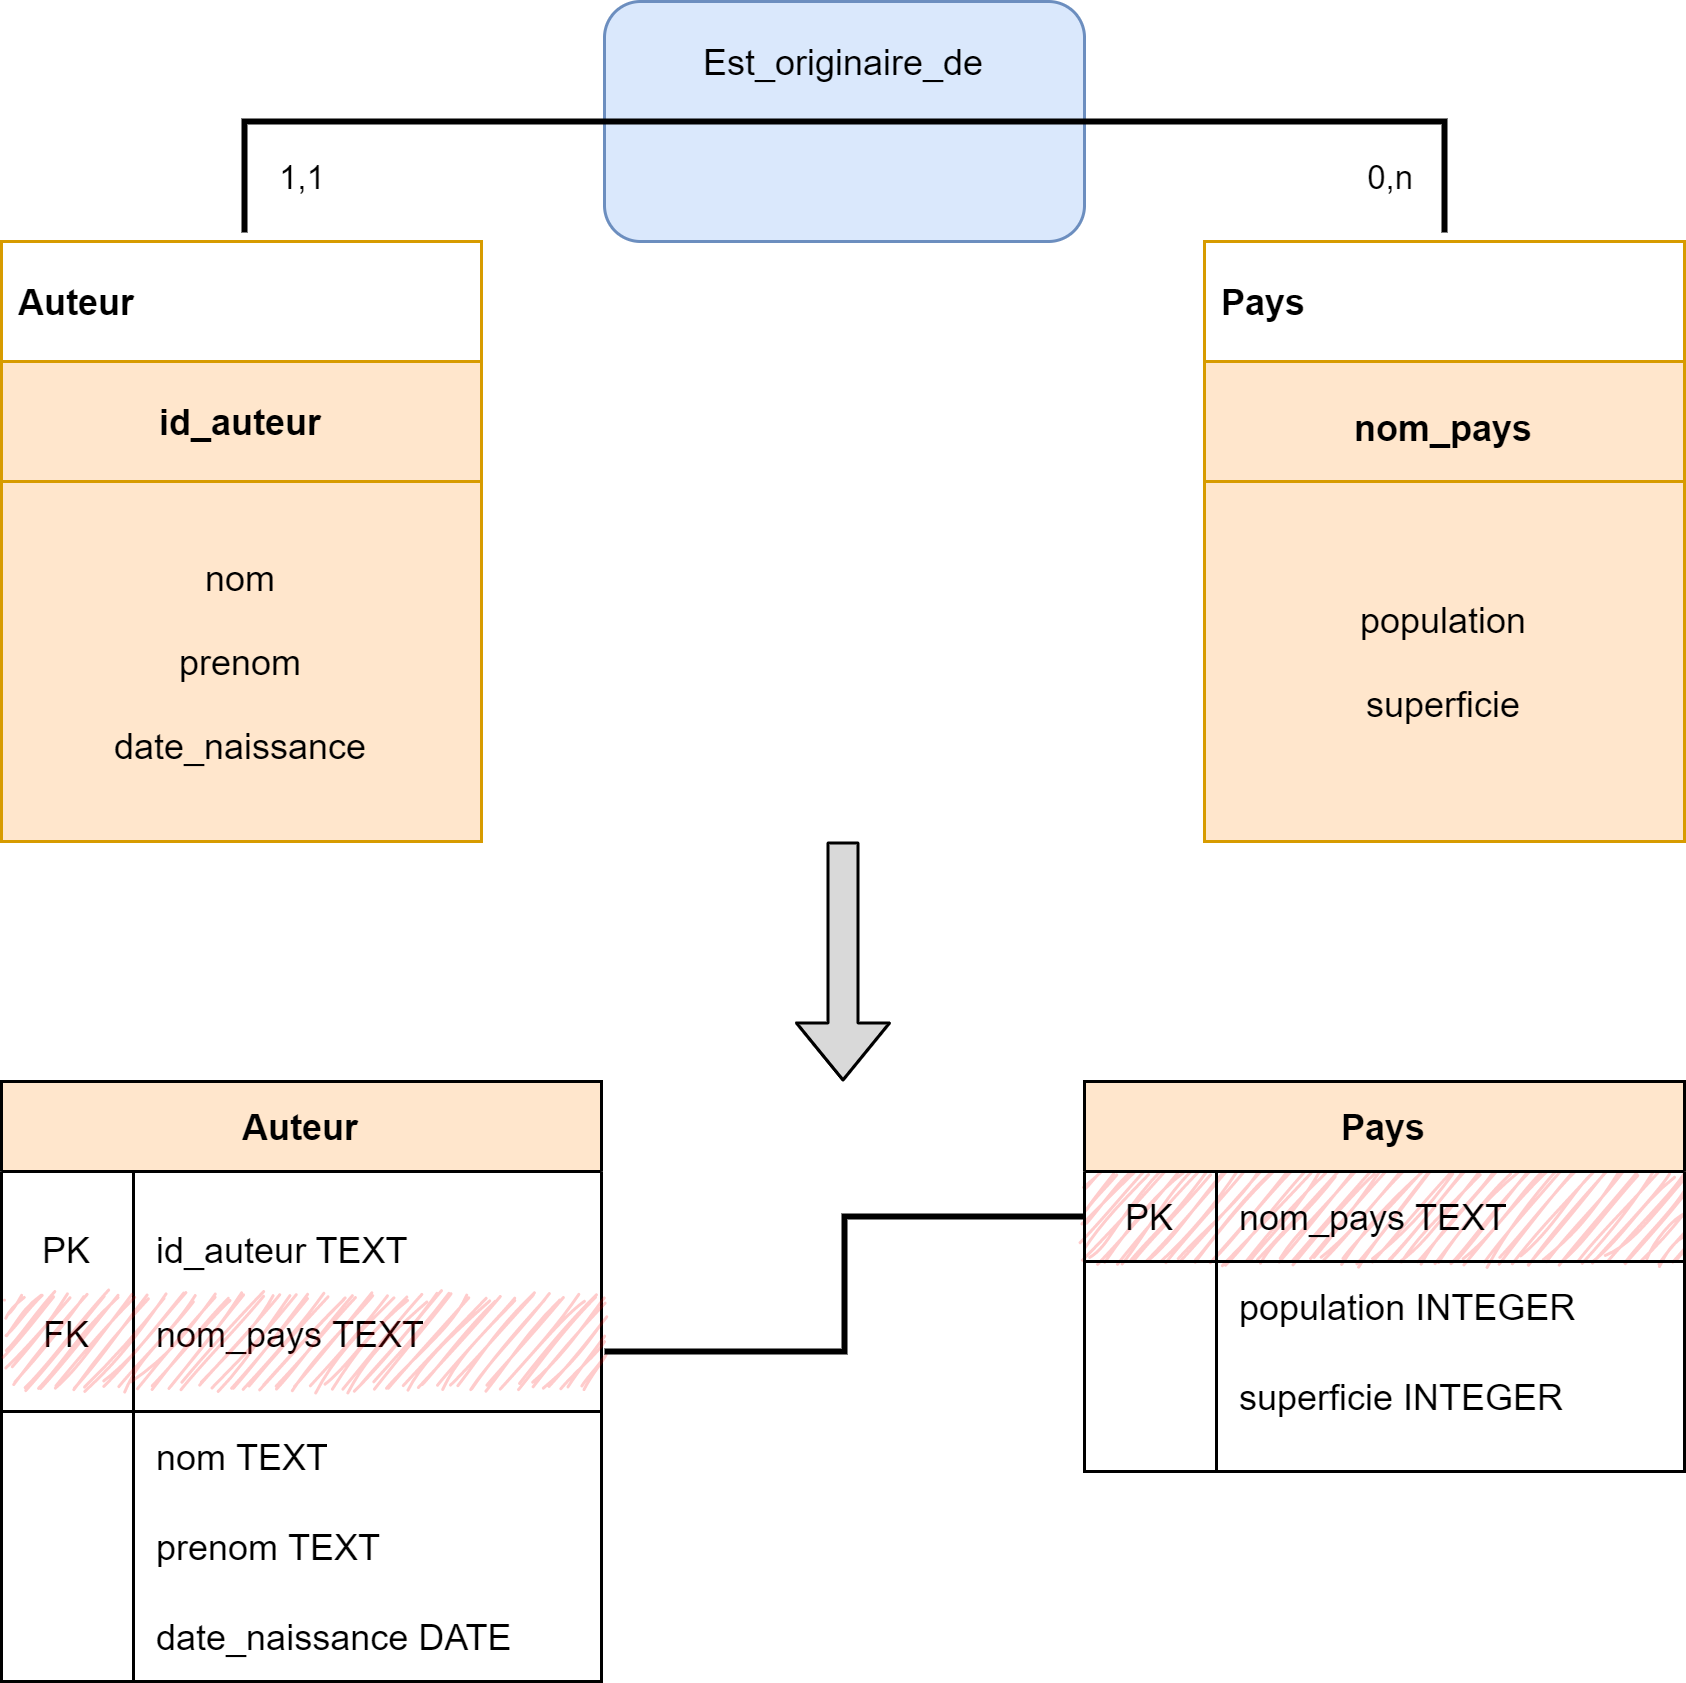
\includegraphics[width=7cm]{img/association_vers_relation_1}
	\end{center}
\end{frame}



\begin{frame}{Transformer une association en relation : cas (0,1) ou (1,1)}

	Puisqu'un auteur vient d'un pays et un seul, on ajoute un attribut nom\_pays à la relation \textbf{Auteur}.

	On précise que cet attribut est \textit{nécessairement} l'un des attributs nom de la relation \textbf{Pays} en ajoutant « FK»  dans le tableau , qui est l'abréviation de \mintinline{sql}{FOREIGN KEY}.

	On dit que nom\_pays est une \alert{clé étrangère}, qui \alert{fait référence} à l'attribut nom de la relation \textbf{Pays}.

	La clé étrangère est soulignée en traits discontinus.\\


	{\footnotesize
		\textbf{Pays}(\uline{nom\_pays TEXT }, population INTEGER, superficie INTEGER)}\\
	{\scriptsize\textbf{Auteur}(\uline{id\_auteur INTEGER}, \dashuline{nom\_pays TEXT} , nom TEXT, prenom TEXTE, date\_naissance DATE)}
\end{frame}

\begin{frame}{Transformer une association en relation : autre cas}
	\alert{Quand la relation ne possède pas de cardinalité valant (0,1) ou (1,1)}
	\begin{center}
		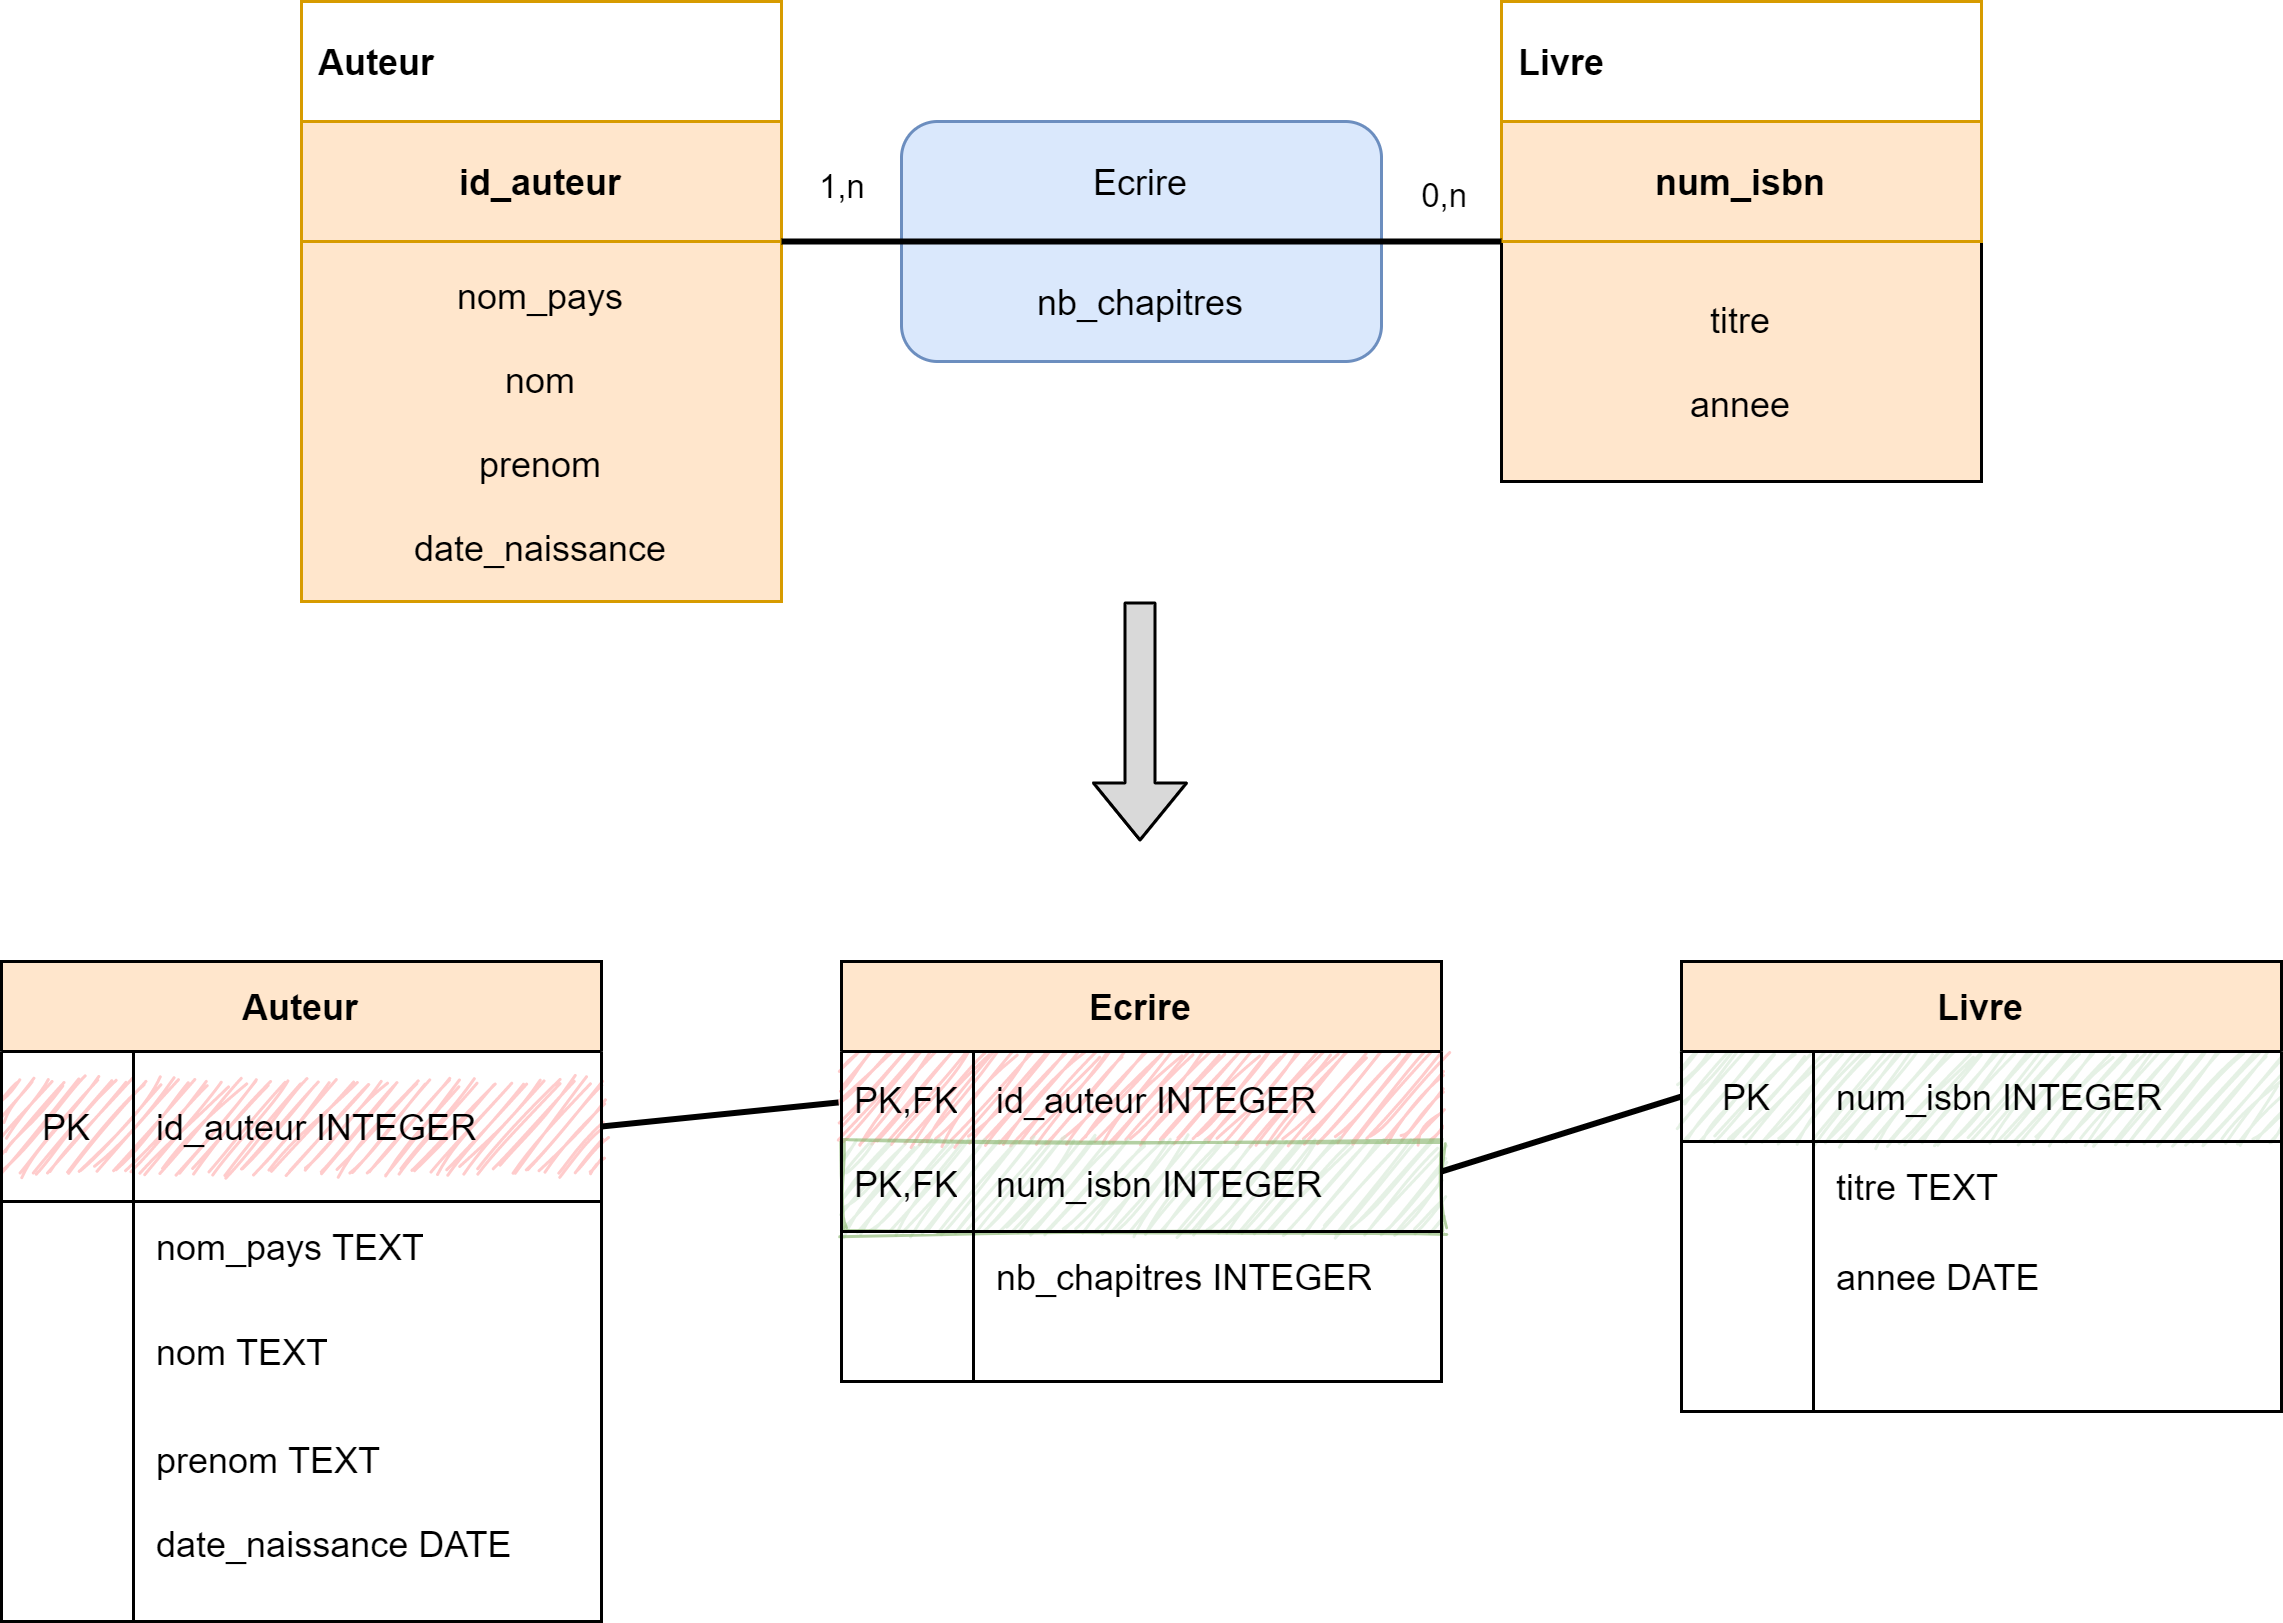
\includegraphics[width=8cm]{img/association_vers_relation_2}
	\end{center}
\end{frame}

\begin{frame}{Transformer une association en relation : autre cas}
	Dans ce cas on fabrique une nouvelle relation :
	\begin{itemize}
		\item on considère les clés primaires des relations issues des entités concernées par l'association;
		\item on fabrique une \alert{nouvelle relation} avec comme clé primaire ce couple de de clés primaires;
		\item ces clés primaires sont également des \alert{clés étrangères};
		\item on ajoute si besoin est d'autres attributs spécifiques à l'association.
	\end{itemize}
	On va noter celaans ce cas on fabrique une nouvelle relation :
	\begin{itemize}
		\item on considère les clés primaires des relations issues des entités concernées par l'association;
		\item on fabrique une \alert{nouvelle relation} avec comme clé primaire ce couple de de clés primaires;
		\item ces clés primaires sont également des \alert{clés étrangères};
		\item on ajoute si besoin est d'autres attributs spécifiques à l'association.
	\end{itemize}
	On va noter cela

	\textbf{Ecrire}(\uline{\dashuline{id\_auteur INTEGER, num\_isbn INTEGER}}, nb\_chapitres INTEGER)\\
\end{frame}
\begin{frame}{Modèle complet}

	{\footnotesize
		\textbf{Pays}(\uline{nom\_pays TEXT }, population INTEGER, superficie INTEGER)\\

		\textbf{Livre}(\uline{num\_isbn INTEGER} , titre TEXT, annee DATE)\\

		{\scriptsize\textbf{Auteur}(\uline{id\_auteur INTEGER}, \dashuline{nom\_pays TEXT} , nom TEXT, prenom TEXTE, date\_naissance DATE)\\}

		\textbf{Ecrire}(\uline{\dashuline{ id\_auteur INTEGER, num\_isbn INTEGER}}, nb\_chapitres INTEGER)}

\end{frame}
\begin{frame}{Remarque}
	Lorsqu'on modélise une BDD, on n'a pas toujours besoin de passer par le MCD pour établir le modèle relationnel : on peut parfois le faire directement.
\end{frame}
\begin{frame}{Bilan}
	Lors qu'on établit un modèle relationnel (à partir d'un MCD ou directement) on définit des relations qui symbolisent des entités ou des associations.

	On définit aussi les \alert{contraintes} de la BDD :
	\begin{itemize}
		\item	\alert{Contraintes de domaines} : c'est essentiellement définir le type des attributs des relations;
		\item	\alert{Contraintes d'entité} : c'est déterminer des clés primaires pour garantir l'unicité de chaque élément d'une relation;
		\item 	\alert{Contraintes de référence} : c'est déterminer les clés étrangères dans les relations;
		\item 	\alert{Contraintes utilisateur} : ce sont des contraintes sur les valeurs des attributs qui garantissent leur cohérence.
	\end{itemize}
\end{frame}
\begin{frame}{Contraintes}
	Ces contraintes vont garantir la cohérence logique de la future base de données
	\begin{itemize}
		\item	à tout instant;
		\item	dans le cas d'une mise à jour des données (insertion ou suppression d'éléments de la relation).
	\end{itemize}
\end{frame}
\begin{frame}{Exemples de contraintes utilisateur}
	Dans la relation \\

	{\footnotesize
		\textbf{Pays}(\uline{nom\_pays TEXT }, population INTEGER, superficie INTEGER)\\}

	On peut rajouter les contraintes utilisateurs suivantes :
	\begin{enumerate}[--]
		\item 	population > 0;
		\item 	superficie > 0.
	\end{enumerate}
	De même dans \textbf{Auteur} et \textbf{Livre} on peut décider que les dates doivent être postérieures à une date donnée.
\end{frame}

\end{document}